\documentclass[a4paper,12pt,titlepage]{article}

\usepackage[pdftex]{graphicx}
\usepackage[headheight=15pt]{geometry}

\usepackage{fancyhdr}
\pagestyle{fancy}
\lhead{Exercises}
\chead{}
\rhead{GIS Basics}

\usepackage[english]{babel}						
\usepackage[utf8]{inputenc}	

\usepackage{array}
\usepackage{colortbl}

\usepackage{listings}
\lstset{language=SQL}
\lstset{frame=single}

\usepackage[section]{placeins}

%PDF hyperlinks
\usepackage[colorlinks=true,linkcolor=orange,bookmarksopen=true,bookmarksnumbered=false,pdfstartpage=2]{hyperref}

\usepackage{color}
\definecolor{orange}{rgb}{1,.5,0}

\title{Exercises: GIS Basics}
\author{Michael Wagner (mwagner@allspatial.info)}      													% 
\date{April 14/15/18, 2016}

\clubpenalty=4500
\widowpenalty=10000
\linespread{1.3}

%%-------------------------Document begins--------------------------------------------
\begin{document}
\maketitle

\tableofcontents
\listoffigures
\lstlistoflistings
\newpage

\section{QGIS installation remark}
QGIS should already be installed on your computers. However, if you want to install it on another computer at a later point take care that there are no spaces in the installation path. So instead of \textit{C:\textbackslash Program Files\textbackslash QGIS Essen} install it under \textit{C:\textbackslash QGIS\_Essen} for example. If there are spaces in the installation path problems might occur during the installation, mostly on computers with Windows XP.

\section{Exercise: Loading data into QGIS and performing basic tasks}

For all exercises you can use the QGIS User Guide as a reference. You will find the user guide in the \textit{Manuals} directory of the \textit{GIS\_Basics} folder.
Start QGIS Desktop. Right-click in the toolbar area and turn of the toolbars you currently don't need (Figure \ref{fig:turn_off_toolbars}).

\begin{figure}[h]
\centering
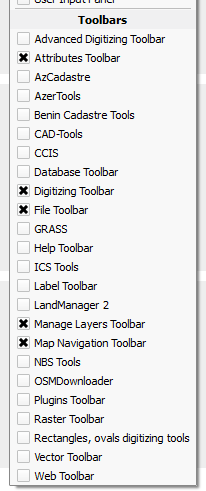
\includegraphics[width=4cm]{Images/turn_off_toolbars.png}
\caption{Turning off toolbars}\label{fig:turn_off_toolbars}
\end{figure}

Use the first button on the \textit{Manage Layers} toolbar to load vector data from a file. Select the \textit{church}, \textit{river}, \textit{district}, \textit{building} and \textit{medical\_facility} Shapefiles from the \textit{Data} directory of the \textit{GIS\_Basics} folder (Figure \ref{fig:load_vector_data}).

\begin{figure}[h]
\centering
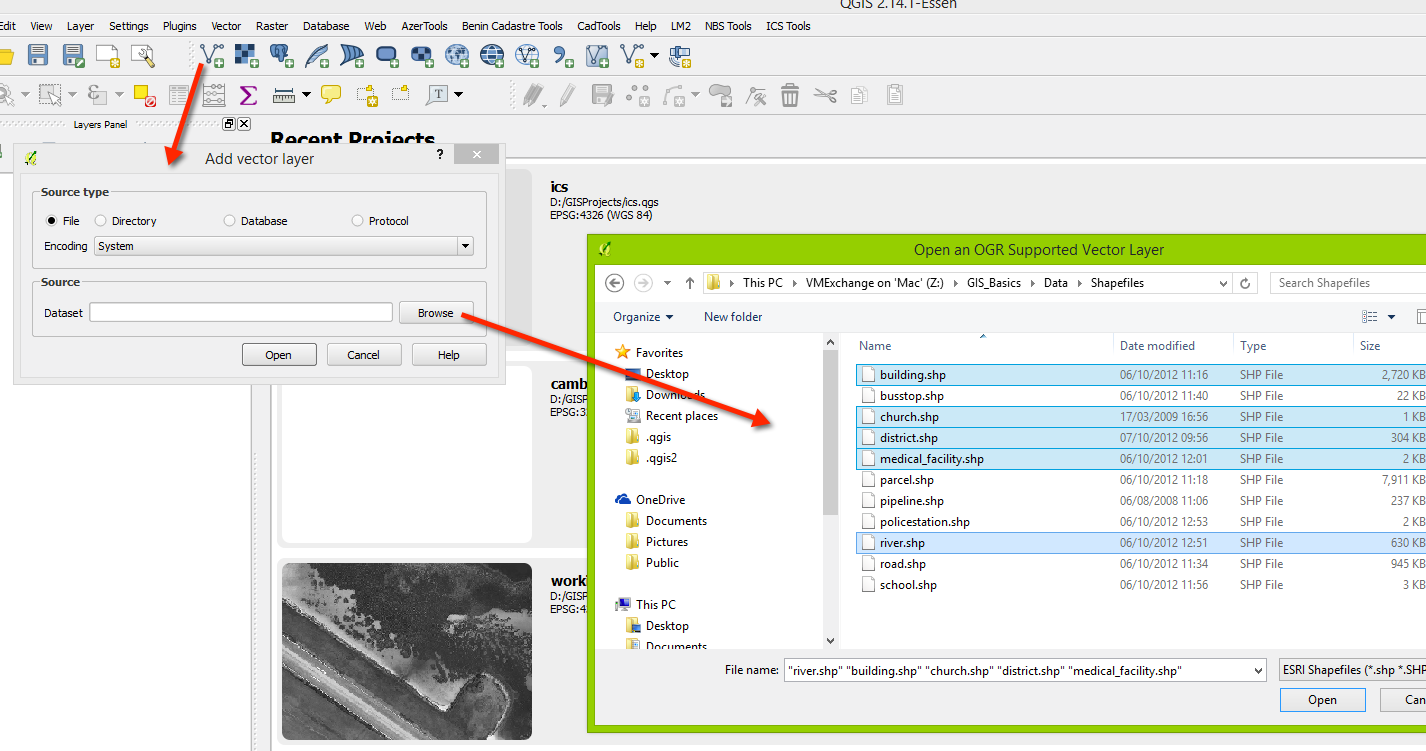
\includegraphics[width=12cm]{Images/load_vector_data.png}
\caption{Loading vector data from Shapefiles}\label{fig:load_vector_data}
\end{figure}

Use the second button on the \textit{Manage Layers} toolbar to load raster data from a file. Select the aerial photo of Mahe (\textit{mahe.ecw}) from the \textit{Data} directory of the \textit{GIS\_Basics} folder. Set the layer's coordinate reference system to EPSG:32740 using the \textit{General} tab of the \textit{Layer Properties} dialog.

Change the order of the layers if you cannot see all layers properly. To do that drag and drop the layers to a different position in the table of contents. Explore the basic tools for map navigation from the relating toolbar (\textit{Map Navigation}). Add a north arrow and a scale bar to your map (Menu \textit{View}:\textit{Decorations}:\textit{North Arrow/Scale Bar}).

\subsection{Changing a layer's layout}

Double-click on a layer in the table of contents to open the \textit{Layer Properties} dialog window.
Click on the \textit{Style} tab to change the layer's style/layout (Figure \ref{fig:layer_properties}). Change the colors, fill styles and symbols according to your likes. Find an appropriate symbol for the \textit{church} layer and the \textit{medical\_facility} layer. Save all the settings and changes you have made so far in a QGIS project (Ctrl+S) in your \textit{GIS\_Basics} folder.

\begin{figure}[h]
\centering
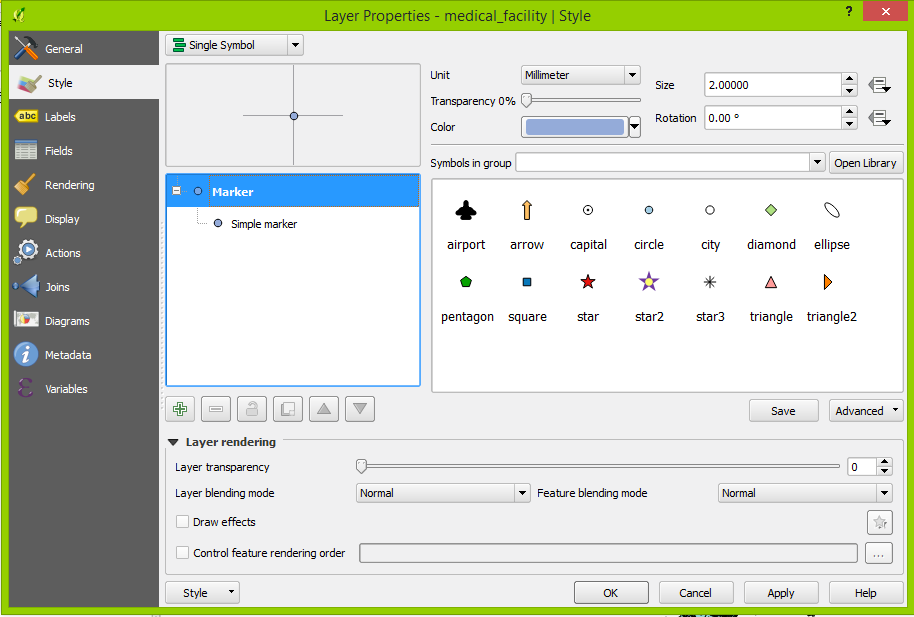
\includegraphics[width=12cm]{Images/layer_properties.png}
\caption{Changing a layer's style}\label{fig:layer_properties}
\end{figure}

\subsection{Labeling a layer}

Label the layers \textit{district} and \textit{river} with their names. Use the \textit{Labels} tab from the \textit{Layer Properties} dialog window (Figure \ref{fig:labelling}). Experiment with the various labeling settings. Make the labeling of the \textit{district} layer scale dependent so that labels are shown only in a scale range from 1:30,000 to 1:150,000.

\begin{figure}[h]
\centering
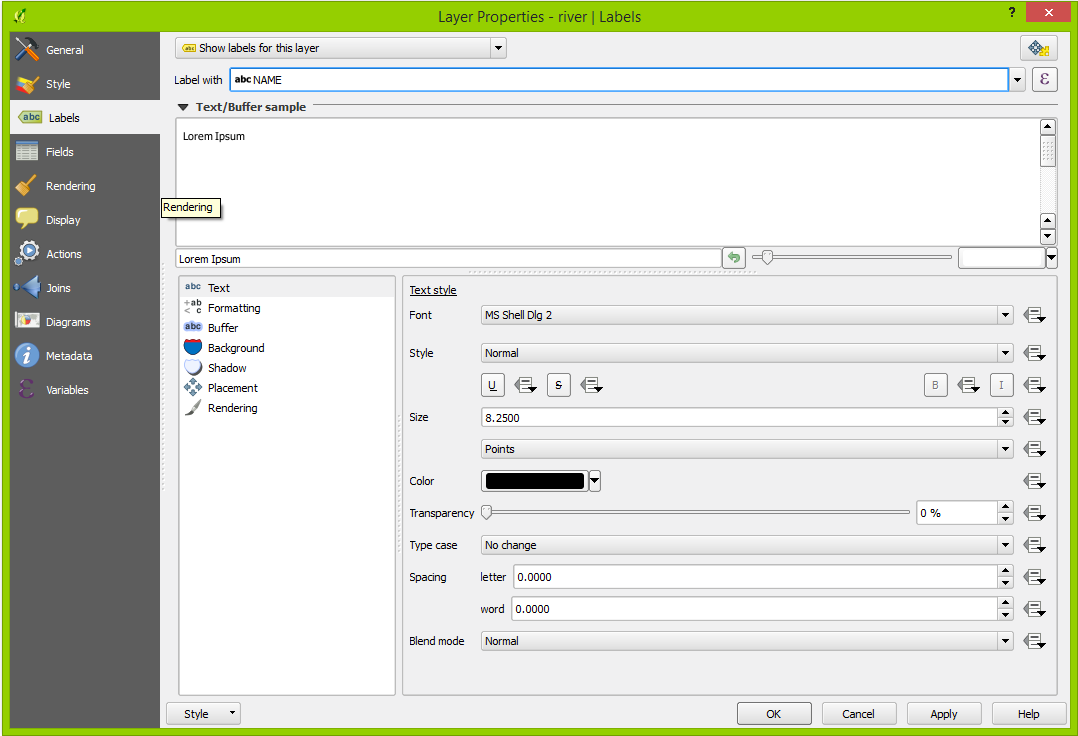
\includegraphics[width=12cm]{Images/labelling.png}
\caption{Labeling a layer's features}\label{fig:labelling}
\end{figure}

\subsection{Loading a raster layer from a Web Map Service}
A Web Map Service (WMS) is a standard web service to provide spatial data through the network in an image format (png, jpg, etc.). The WMS is an ISO (International Organization for Standardization) standard and an OGC (Open Geospatial Consortium) standard. All current GIS software supports consumption of data from a WMS including QGIS. The Centre for GIS (MLUH) configured a WMS to provide the aerial photo and other layers. Provided that you have an Internet connection you can use the WMS of the MLUH to load the aerial photo as a background layer in addition to your existing layers.

From the \textit{Manage Layers} toolbar click the \textit{Add WMS/WMTS Layer} button. Click the \textit{New} button to register the connection to a new WMS (Figure \ref{fig:wms}).

\begin{figure}[h]
\centering
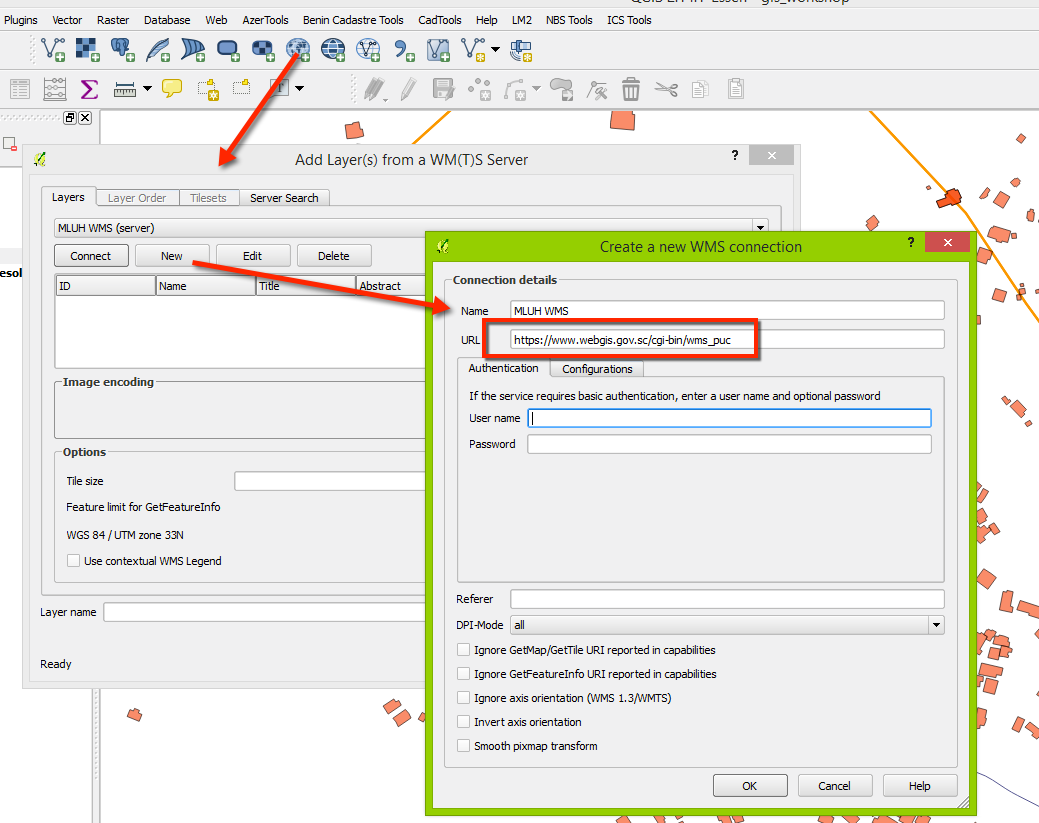
\includegraphics[width=12cm]{Images/wms.png}
\caption{Registering a new WMS connection}\label{fig:wms}
\end{figure}

Connect to the WMS by clicking the \textit{Connect} button. You should see a list of layers that this service provides. Select the \textit{aerial\_photo} layer and click the \textit{Add} button (Figure \ref{fig:wms2}). A new layer will appear in the table of contents. Move the layer to the bottom so it won't cover other layers.

\begin{figure}[h]
\centering
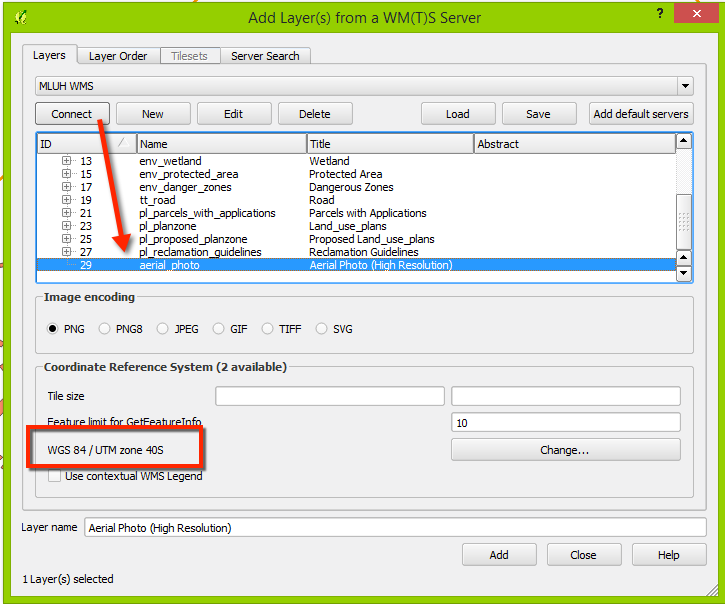
\includegraphics[width=12cm]{Images/wms2.png}
\caption{Connecting to the WMS}\label{fig:wms2}
\end{figure}

\subsection{Creating a thematic map}

Thematic maps are used to show trends or patterns in your data. We will create a thematic map that shows the percentage of  persons injured by fire incidents per district. The dataset is a fictive one but might be similar to records the SFRSA maintains. You find the prepared dataset in the file \textit{fire\_incidents\_2015.csv} in the \textit{Data\textbackslash FireIncidents\textbackslash CSV} directory of the \textit{GIS\_Basics} folder. Open the file with the text editor \textit{Notepad++} and try to understand its structure. We will join that data with the \textit{district} Shapefile.

\subsubsection{Joining a layer with data from a text file}
Load the \textit{fire\_incidents\_2015.csv} file into QGIS with the \textit{Add Vector Layer} tool. The tool's name might be a bit confusing in that case since we will load attribute data only but not a real vector layer. From the file type filter select \textit{Comma Separated Value (*.csv)}. When we join a layer's data with data from a text file we need to have a column in both datasets that contains the same information, usually some ID, number, code, etc. Find out which are the columns we can use to join the \textit{district} layer and the \textit{fire\_incidents\_2015.csv} text file.
Double-click the \textit{district} layer in the table of contents and go to the \textit{Joins} tab. Click the \textit{+} button to add a new join. Configure the fields as shown in Figure \ref{fig:join}.

\begin{figure}[h]
\centering
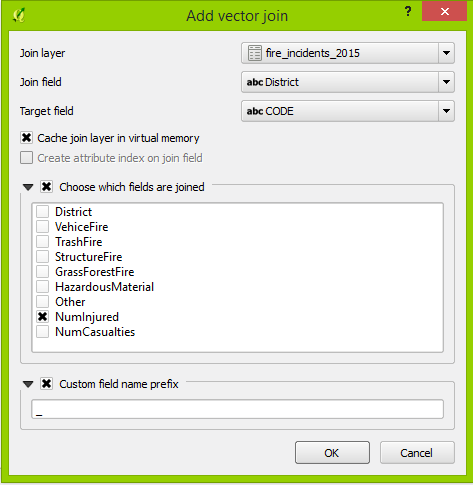
\includegraphics[width=12cm]{Images/join.png}
\caption{Joining a layer with a text file}\label{fig:join}
\end{figure}

Close all dialog windows by clicking the relating \textit{OK} button. Open the attribute table of the \textit{district} layer (Right-click on the layer and select \textit{Open Attribute Table}). The table should now have one new column coming from the \textit{fire\_incidents\_2015.csv} text file. A join is kept in memory and is temporary only. That is why we will save the layer to a new Shapefile \textit{district\_and\_fire\_data.shp}. Right-click the layer and select \textit{Save As...}. Save the new Shapefile in the \textit{Shapefile} directory under the \textit{Data} folder (Figure \ref{fig:save_to_shapefile}).

\begin{figure}[h]
\centering
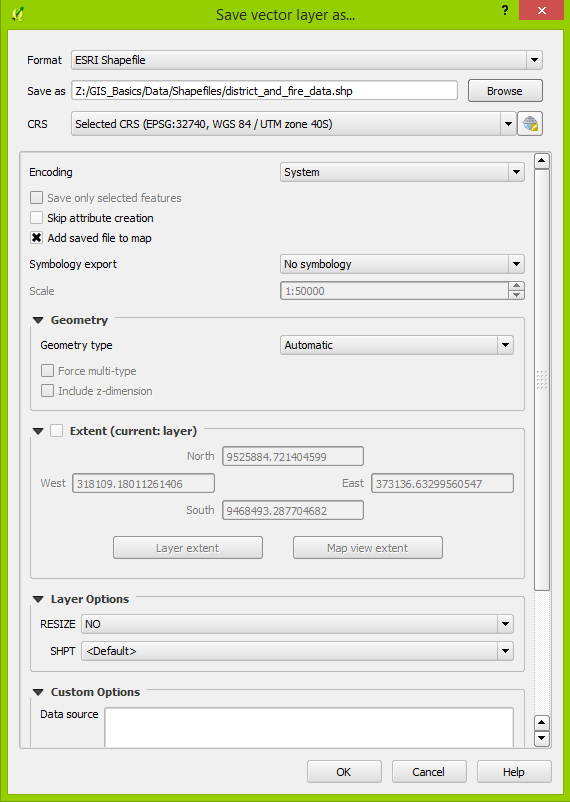
\includegraphics[width=6cm]{Images/save_to_shapefile.png}
\caption{Saving a layer to a Shapefile}\label{fig:save_to_shapefile}
\end{figure}

If you toggled the \textit{Add saved file to map} box the new Shapefile will be added as a layer to QGIS automatically. Remove the original \textit{district} layer and the \textit{fire\_incidents\_2015} layer from the table of contents and save your QGIS project.

\subsubsection{Coloring the districts based on the number of injured persons}
Double-click the \textit{district\_and\_fire\_data} layer and go to the \textit{Style} tab. From the drop-down list in the upper left corner select \textit{Graduated} instead of \textit{SingleSymbol}. The column on which we want to base our thematic map is \textit{\_NumInjure}.
Select a color ramp of your choice and five classes (Figure \ref{fig:thematic1}).

\begin{figure}[h]
\centering
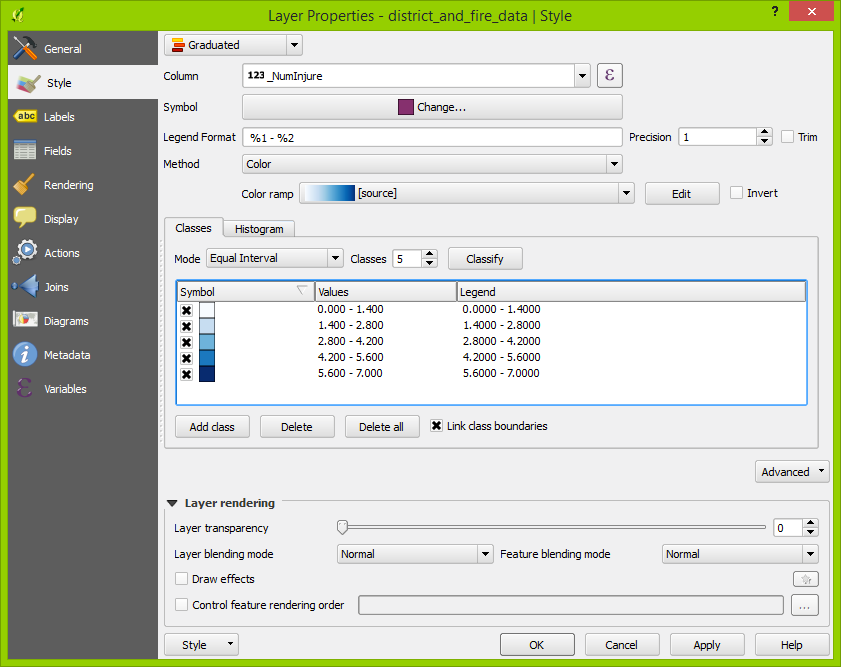
\includegraphics[width=10cm]{Images/thematic1.png}
\caption{Creating a thematic map}\label{fig:thematic1}
\end{figure}

The absolute number of injured persons is not too useful for our purpose. What would actually be a better figure is the percentage of injured diagnosed persons per district. This is a number that is appropriate to compare data.

\subsubsection{Adding a new column to a layer and populating it}
We will add a new column to the layer \textit{district\_with\_fire\_data} to hold the percentage of injured people. Open the attribute table of the layer and click the \textit{Open field calculator} button (It's the last one on the toolbar). The \textit{Field calculator} dialog will open.
We will create a new field/column of type \textit{decimal number} with a precision of 2 and call it \textit{INJU\_PERC}. Add the expression/formula as show in Figure \ref{fig:field_calculator}.

\begin{figure}[h]
\centering
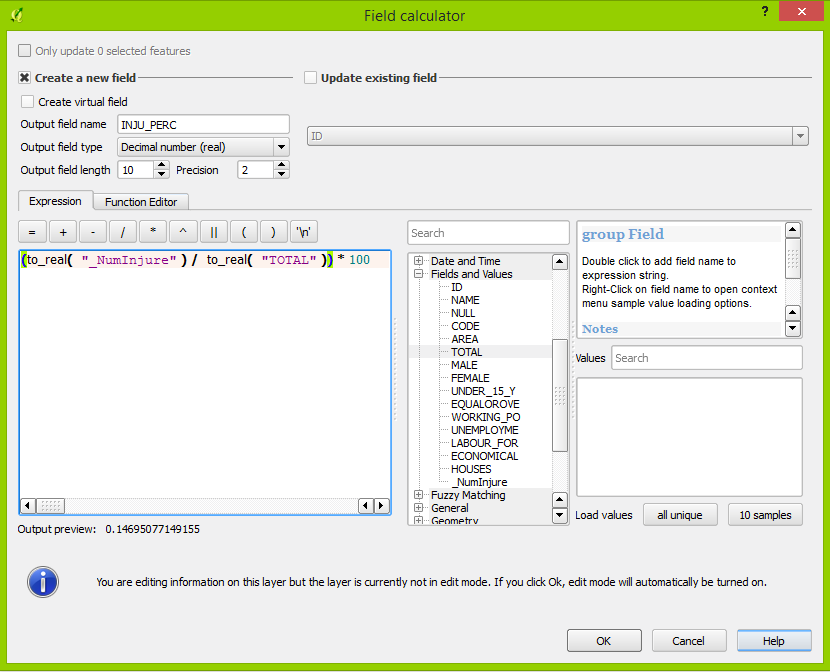
\includegraphics[width=10cm]{Images/field_calculator.png}
\caption{Field Calculator Dialog}\label{fig:field_calculator}
\end{figure}

Click OK to close the dialog and perform the calculation and population. Stop editing by clicking the button with the yellow pencil and save your changes. Close the attribute table and create a thematic map, this time based on the percentage of injured persons per district. What are the three districts with the highest percentage?

\subsubsection{Adding a diagram to your map}
You can also add a pie chart diagram to your map to show the relation of different types of fire incidents. Load the \textit{district} and \textit{fire\_incidents\_2015} layers again and create a join on layer \textit{district} as in the previous exercise. Select \textit{VehicleFire}, \textit{StructureFire} and \textit{GrassForestFire} as the fields to be included in the join. Open the \textit{Layer Properties} dialog of the \textit{district} layer and click the \textit{Diagrams} tab. Make the settings as shown in Figure \ref{fig:diagram}. Your final thematic map could look like Figure \ref{fig:thematic_final}.

\begin{figure}[htb]
\centering
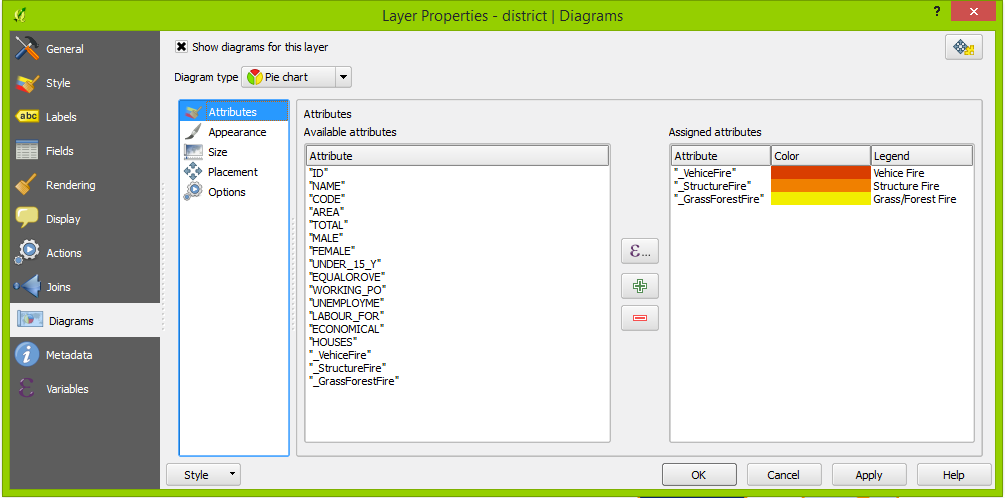
\includegraphics[width=11cm]{Images/diagram.png}
\caption{Configuring a diagram}\label{fig:diagram}
\end{figure}

\begin{figure}[htb]
\centering
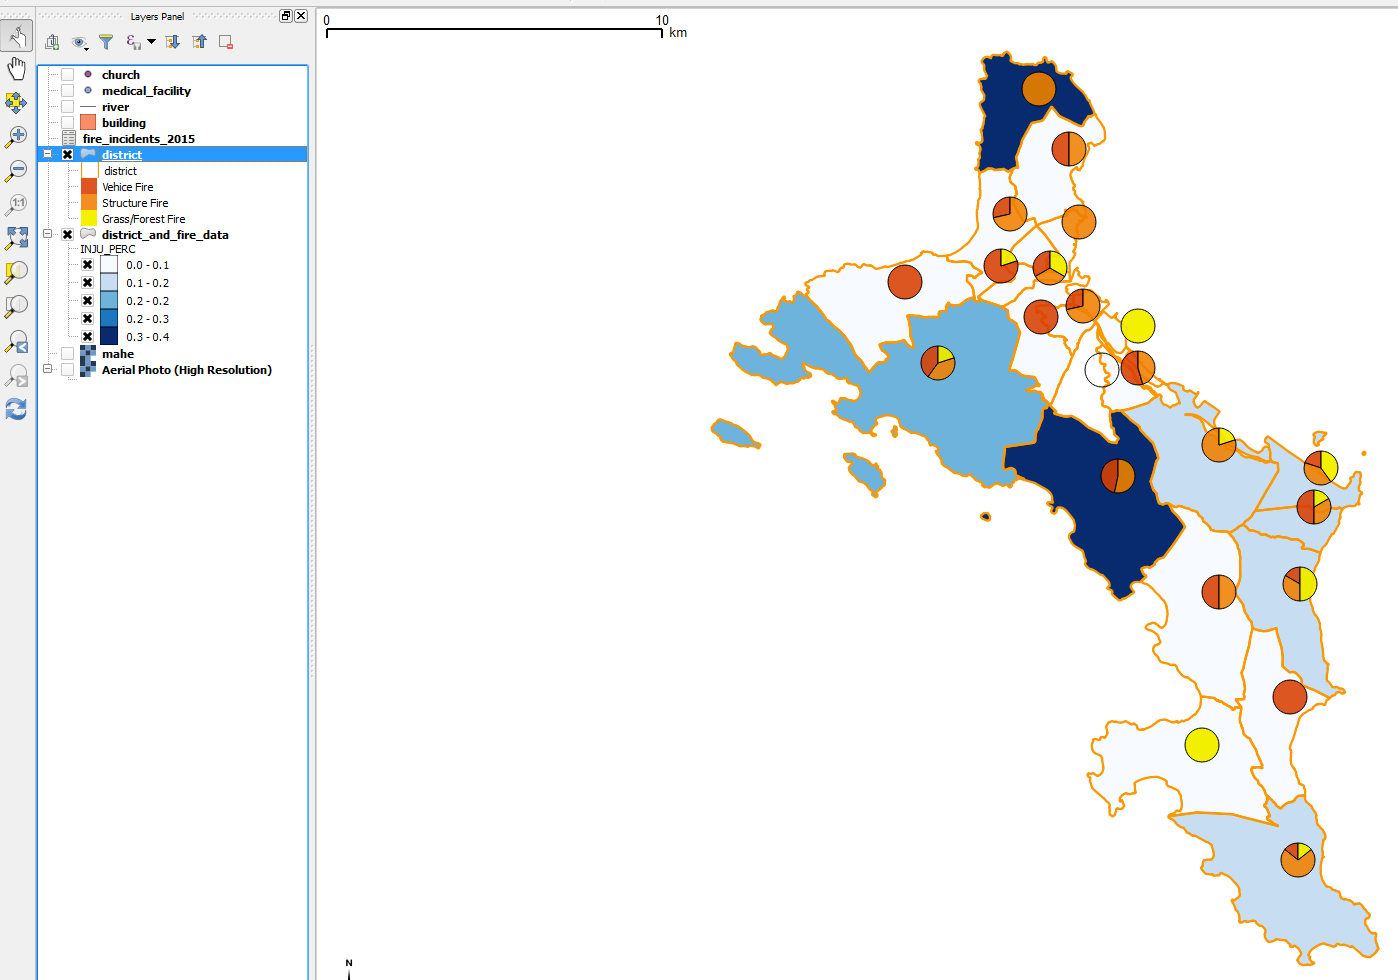
\includegraphics[width=12cm]{Images/thematic_final.png}
\caption{The thematic map, finalised}\label{fig:thematic_final}
\end{figure}

\subsubsection{Practising the creation of thematic maps}
Create two more thematic maps that will show the percentage of casualties and structure fires in fire incidents. Use the original \textit{district} Shapefile and \textit{fire\_incidents\_2015} CSV file again. The final result should be these new layers:

\begin{itemize}
\item \textit{district\_and\_casualties}
\item \textit{district\_and\_structure\_fires}
\end{itemize}

Create the second map/layer only after going through the \textit{Performing spatial queries} Chapter. 

%-------------------------------------------------------------------------

\section{Exercise: Performing attribute queries}
In QGIS you can perform attribute queries in two ways, each one for a different purpose. You can right-click on a (vector) layer in the table of contents and select \textit{Filter...}. You can then define a filter condition in the \textit{Query Builder} dialog that will open. Only those features that match this filter will be loaded from the dataset. Performing a query this way is perfect if you want to load only a subset of a layer's data because it is a very large dataset for example.
Your can try the filter expression as follows to show only those districts from the \textit{district} layer whose name starts with \textit{A}:

\begin{lstlisting}[caption={Filter districts whose name starts with \textit{A}},label=lst:districts_with_a]
"NAME" LIKE 'A%'
\end{lstlisting}

The second way to perform an attribute query is from within the attribute table of a (vector) layer.
A similar dialog will open where you can define a filter expression/condition. The difference is that those features matching the filter condition will be selected among all features in that layer but still all features will be available (Figure \ref{fig:filter1}). You can then extract the selected features and/or use them for further analysis/processing.

\begin{figure}[htb]
\centering
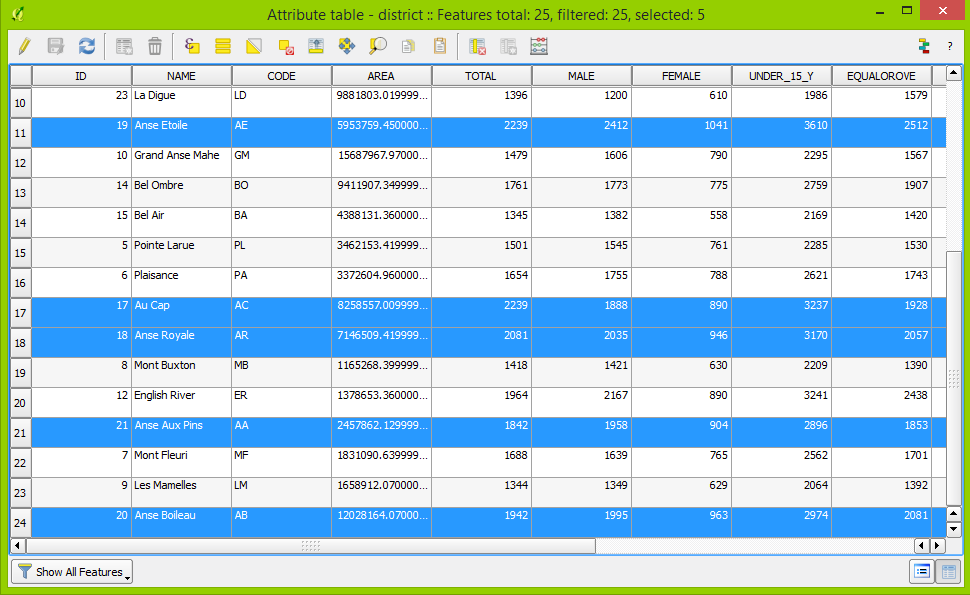
\includegraphics[width=12cm]{Images/filter1.png}
\caption{Districts with \textit{A...} selected among all districts}\label{fig:filter1}
\end{figure}

To save only the selected features of a layer you can use the \textit{Save As...} command from the layer's context menu and toggle the \textit{Save only selected features} checkbox in the resulting dialog window.

\subsection{Exporting query results to be viewed in Google Earth}
QGIS also supports storing spatial data in KML (Keyhole Markup Language) format (Figure \ref{fig:kml}). KML is the file format used by Google Earth and Google Maps. You could for example save the previously selected districts to KML and then just double-click the KML file you created (in the Windows Explorer) to start Google Earth. Google Earth will zoom to the Seychelles and nicely overlay the districts with its satellite images or aerial photos, etc. 

\begin{figure}[htb]
\centering
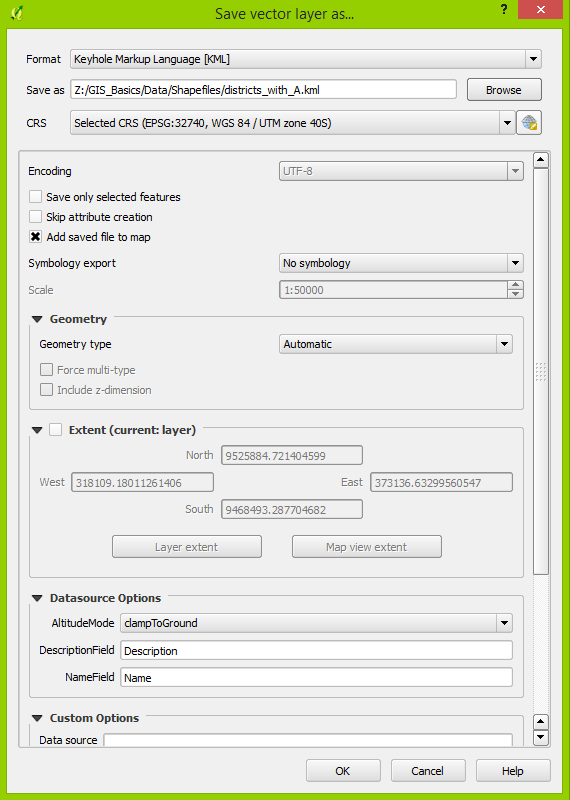
\includegraphics[width=6cm]{Images/kml.png}
\caption{Saving data to a KML file}\label{fig:kml}
\end{figure}

\subsection{Practising attribute queries}
Try to answer the following questions using attribute queries. Save the query results (the selected features) to separate Shapefiles and name the files accordingly.

\begin{itemize}
\item Which are the districts with more than 2000 inhabitants? (Layer:district, Attribute:TOTAL) 
\item Which are the districts where the number of casualties in fire accidents was higher than the number of injured persons? (Layer:district joined with layer fire\_incidents\_2015, Attributes:NumInjured, NumCasualties)
\item How many churches are Catholic churches? (Layer:church, Attribute:TYPE)
\item Which are the rivers with a length of more than 2000 meters? (Layer:river, Attribute:LENGTH)
\item How many parcel where created after January 1, 2003 and have an area larger than 5000 square meters? (Layer:parcel, Attributes:AREA, VALIDFROM)
\end{itemize}

%------------------------------------------------------

\section{Exercise: Performing spatial queries}
Spatial queries are based on the spatial relationship of features and are one of the most powerful capabilities of GIS. The spatial query tool of QGIS you will find under the menu \textit{Vector}:\textit{Spatial Query}. Based on the spatial operator/filter that you choose certain features will be selected as a result of the spatial query similar to those selected by an attribute query. The selected features you can then save in a separate file/layer again and/or use for further queries/processing.
For most of the analysis that you do you will use spatial and attribute queries in a combined way and the result of an attribute query might be used as input for a spatial query (or vice versa). If we wanted to find the health facilities in Anse Royale we could first perform an attribute query to select the district with \textit{NAME = 'Anse Royale'} and then use the result of this query as input for a spatial query (Figure \ref{fig:spatial_query1}).

\begin{figure}[h]
\centering
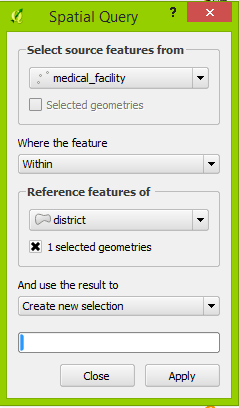
\includegraphics[width=6cm]{Images/spatial_query1.png}
\caption{Performing a spatial query}\label{fig:spatial_query1}
\end{figure}

\subsection{Buffers/Buffer Zones}
Buffers are very useful and required as input for many spatial queries. A buffer is an area/polygon around a feature that is created based on the buffer distance you define. In QGIS you can create a buffer using the \textit{Buffer(s)} tool from the \textit{Vector:Geoprocessing Tools} menu. If the the Anse Royale District is still selected from the previous attribute query you can create a buffer zone just around this district using the settings as shown in Figure \ref{fig:buffer}.

\begin{figure}[h]
\centering
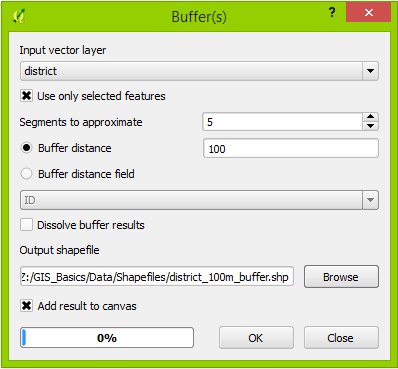
\includegraphics[width=8cm]{Images/buffer.png}
\caption{Creating a buffer around the selected feature(s) of the \textit{district} layer}\label{fig:buffer}
\end{figure}

\subsection{Practising spatial queries}
Use your knowledge on spatial (and attribute) queries to answer the following questions. You will need a combination of several queries to find answers to most of the questions. Save each final result to a Shapefile.

\begin{itemize}
\item Which are the parcels within 100 meters of \textit{Riviere Anse Louis} that have a size  between 3000 and 8000 square meters?
\item Which are the buildings within 1500 meters of \textit{Beoliere Hospital} as well as within 1500 meters of \textit{Souvernir Health Centre}?
\item Which are the buildings in \textit{Baie Lazare} that are not within 1500 meters of any governmental hospital/clinic?
\item Which are the schools that have no bus stop within a distance of 200 meters?
\item Which land (parcels) is crossed by \textit{Riviere Bon Espoir}?
\item Which are the neighbour districts of Anse Boileau?
\end{itemize}


\section{Exercise: Creating and editing data}
In this exercise you will create a new Shapefile layer. Let's say you need a layer to capture fire incident locations and the relating details. The location could be represented by a point geometry and the attributes you need could be those:

\begin{itemize}
\item ID
\item INCIDENT\_DATE
\item INCIDENT\_TYPE
\item INCIDENT\_CAUSE
\item NO\_INJURED
\item NO\_CASUALTIES
\end{itemize}

Add any other attribute that you consider useful/important. Select the \textit{New Shapefile Layer...} tool from the \textit{Layer}:\textit{Create Layer} menu. Create the attributes and set the appropriate data type accordingly (Figure \ref{fig:create_shapefile_layer}). Be aware that attribute names in Shapefiles cannot be longer than 10 characters, so you have to find some abbreviation for your field names. Once you created all the required attributes click \textit{OK} and save the Shapefile as \textit{fire\_incident.shp}.

\begin{figure}[htb]
\centering
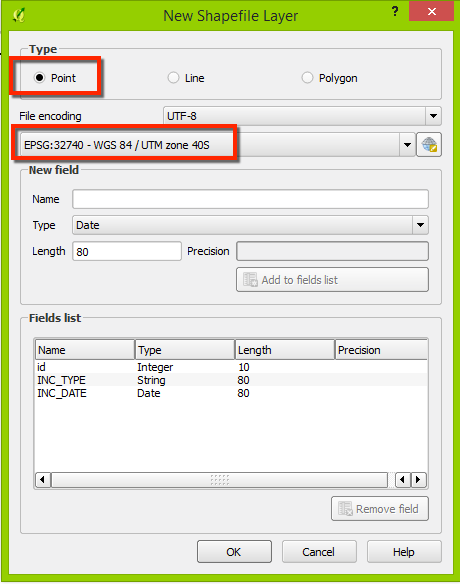
\includegraphics[width=6cm]{Images/create_shapefile_layer.png}
\caption{Creating a Shapefile layer}\label{fig:create_shapefile_layer}
\end{figure}

You can then select the new layer in the table of contents and \textit{Toggle Editing} from the layer's context menu. The \textit{Digitizing} toolbar will be activated and you can select the \textit{Add Feature} tool to capture the fire incident locations. Create five fictive locations and enter the attributes in the dialog that will pop up for each new location (Figure \ref{fig:create_features}).

\begin{figure}[htb]
\centering
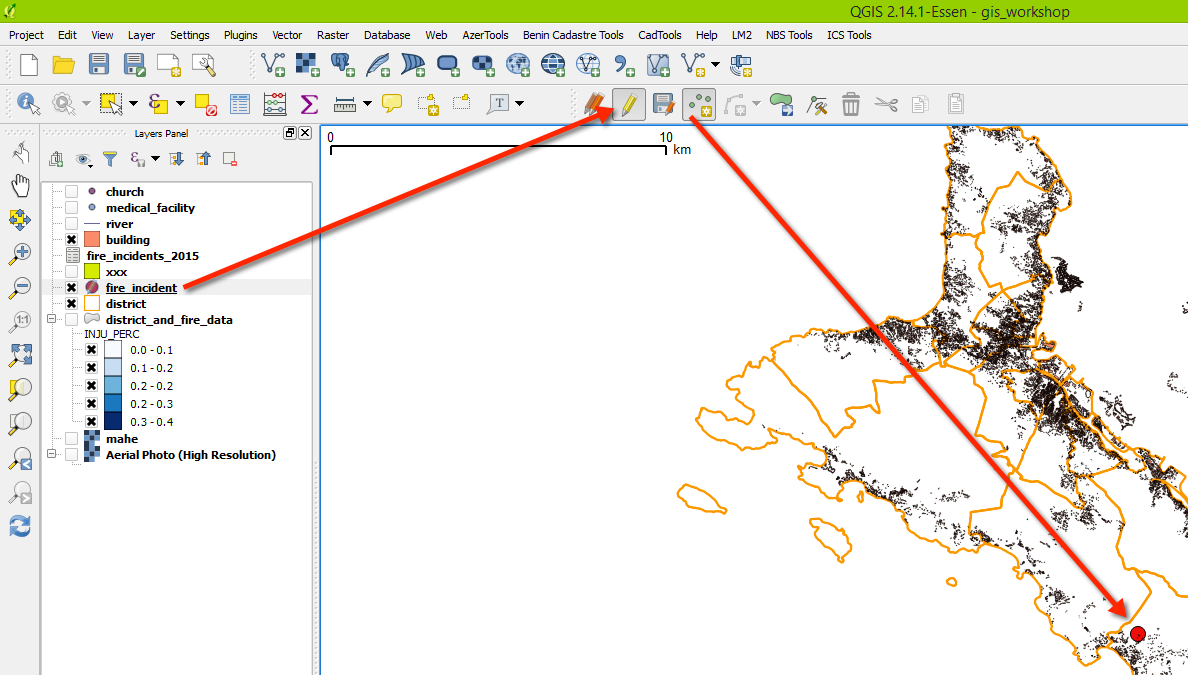
\includegraphics[width=12cm]{Images/create_features.png}
\caption{Capturing fire incident locations}\label{fig:create_features}
\end{figure}

Once you are done capturing the incident locations you can select \textit{Toggle Editing} from the layer's context menu again to finish the editing and save your work.

If the incident locations came from a GPS measurement you can load the text file containing the GPS coordinates into QGIS and then create the new features in your \textit{fire\_incident} layer by snapping the points you create to the GPS points from the text file. Use the \textit{Add Delimited Text Layer} tool from the \textit{Layer} menu and select the \textit{incident\_coordinates.csv} file from the \textit{FireIncidents} directory in the \textit{Data} folder (Figure \ref{fig:load_csv}). After loading the layer set the coordinate reference system to EPSG:32740 in the \textit{General} tab of the \textit{Layer Properties} dialog.

\begin{figure}[htb]
\centering
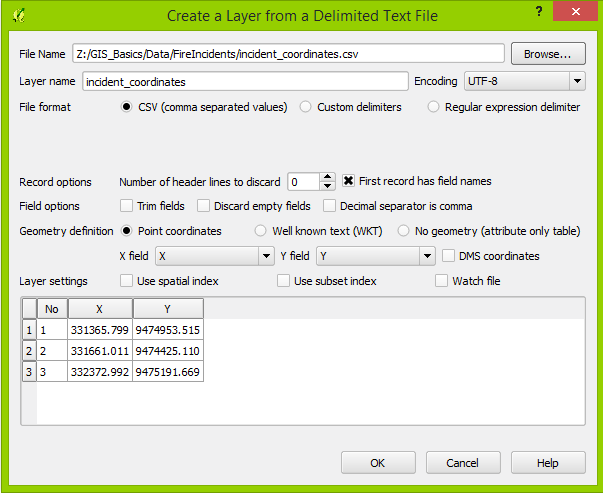
\includegraphics[width=8cm]{Images/load_csv.png}
\caption{Loading vector data from a delimited text file}\label{fig:load_csv}
\end{figure}

Open the \textit{Snapping Options} dialog from the \textit{Settings} menu and set the snapping tolerance for the \textit{incident\_coordinates} layer to 10-20 meters (Figure \ref{fig:snapping_tolerance}).

\begin{figure}[htb]
\centering
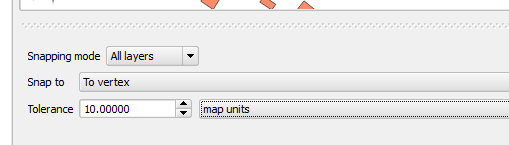
\includegraphics[width=10cm]{Images/snapping_tolerance.png}
\caption{Setting the snapping tolerance}\label{fig:snapping_tolerance}
\end{figure}

Then toggle editing for the \textit{fire\_incident} layer and use the \textit{Add Feature} tool to capture new points. When you set the new points just move the mouse pointer somewhere near the points from the \textit{incident\_coordinates} layer and QGIS will snap the new points precisely. Create the three point features, enter their attributes (just come up with some fictive data) and save your changes.

\section{Exercise: Preparing a map for printing}
Sometimes you need to create a map to be printed on paper, to an image file or to a PDF file. Such a map should have a legend as well as a north arrow and scalebar. QGIS has a \textit{Print Composer} to create such maps. Select the \textit{New Print Composer} tool from the \textit{File} menu. The Print Composer lets you build a map layout and add the required components (scalebar, legend, attribute data, etc.).
Create a nice map layout for one of the thematic maps that you created in the previous exercises. The result could look as in Figure \ref{fig:map_layout}.

\begin{figure}[htb]
\centering
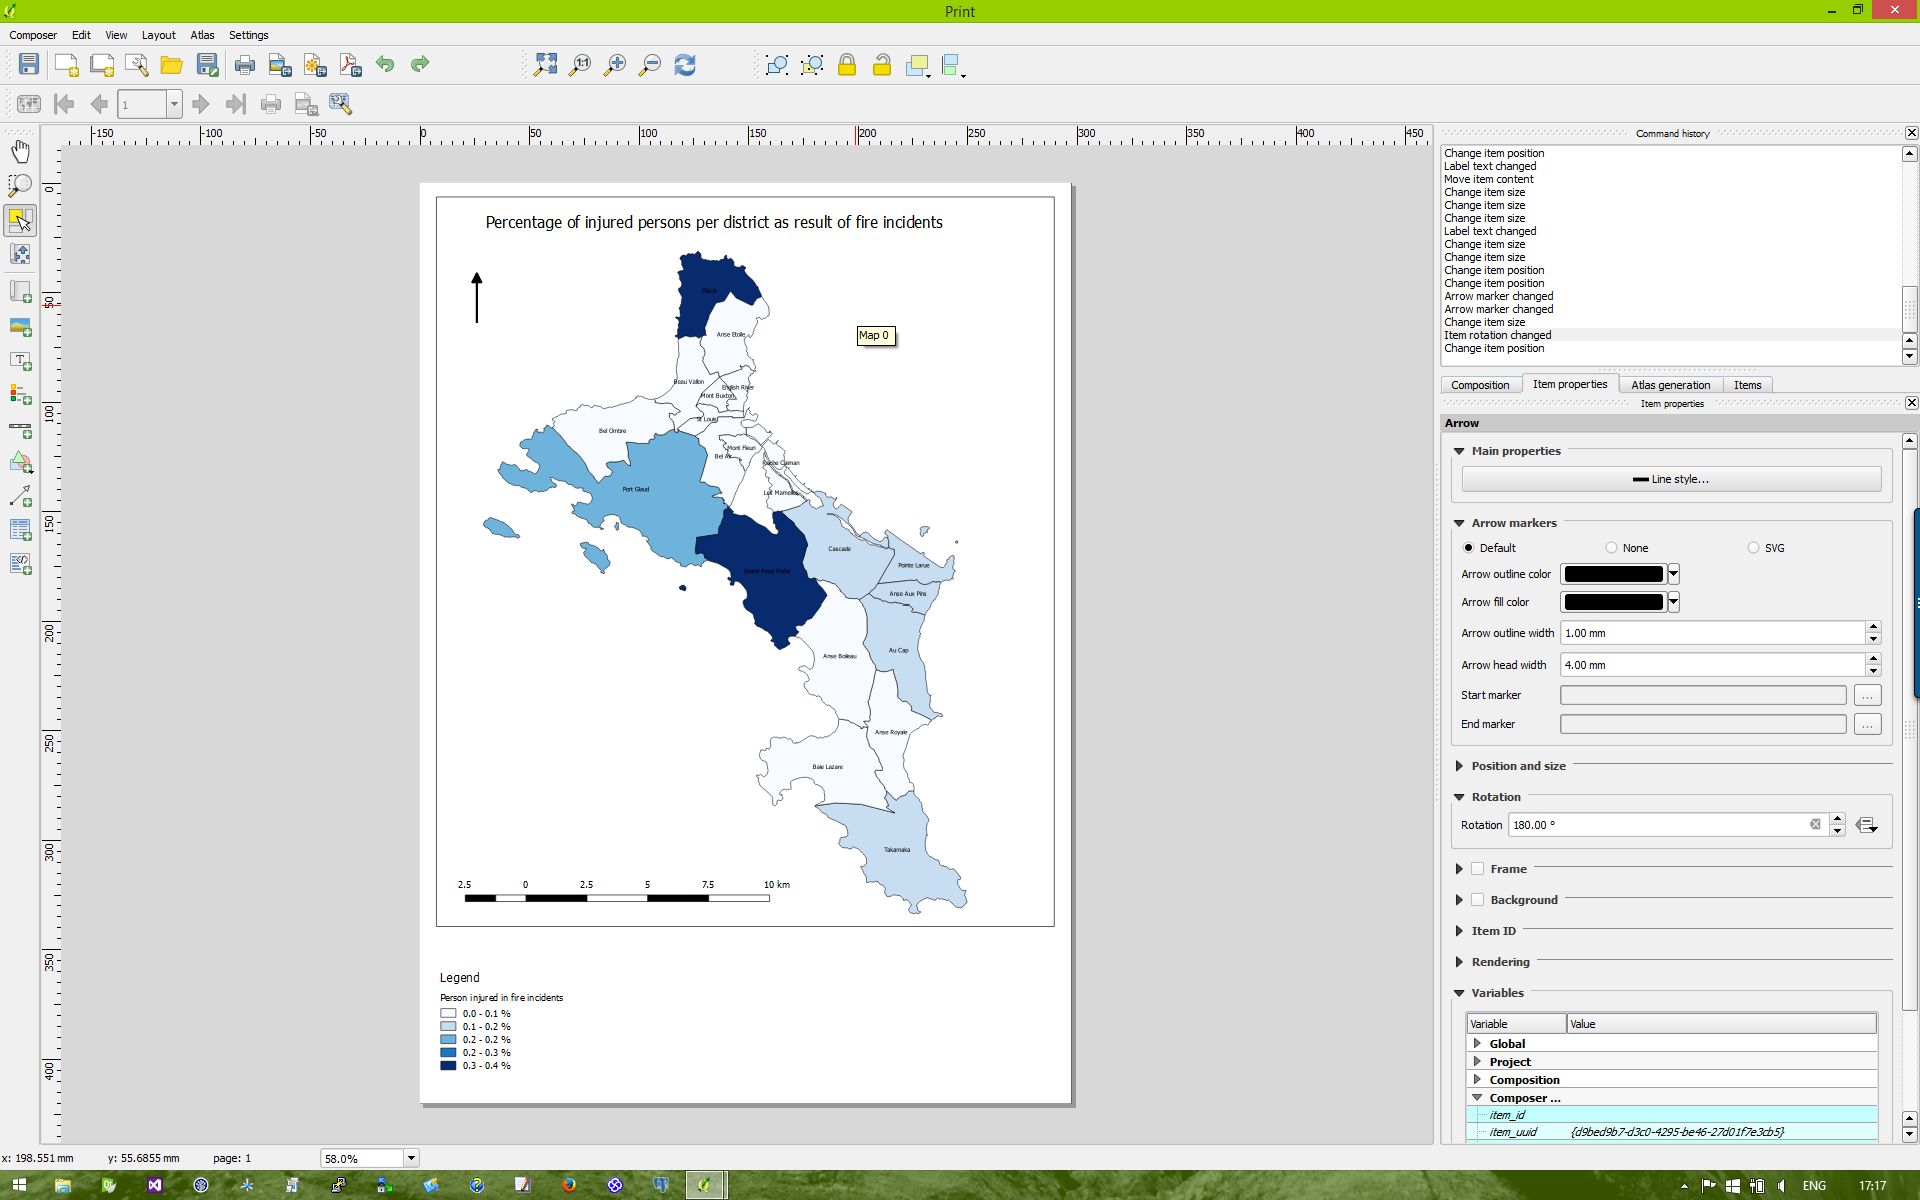
\includegraphics[width=14cm]{Images/map_layout.png}
\caption{Creating a print map layout}\label{fig:map_layout}
\end{figure}

\end{document}
